\section{Objectgeori\"enteerd Programmeren}

\frame{ \tableofcontents[currentsection] }

\begin{frame}
  \frametitle{Context}
  \begin{itemize}
    \item Software wordt alsmaar complexer en omvangrijker
    \item Complexiteit moet onder controle gehouden worden
    \item Structuur nodig
  \end{itemize}
  \begin{center}
    \begin{tabular}{lr}
      {\bf Software} & {\bf Lines of code} \\
      \hline
      Gimp & 732,000 \\
      \NODE{\href{http://en.wikipedia.org/wiki/Unreal_Engine}{\beamergotobutton{Unreal Engine}}}{unreal} & 2,000,000 \\
      Firefox & 9,500,000 \\
      Linux Kernel (3.10) & 15,800,000 \\
      % Windows NT 3.1 & 4,000,000 \\
      % Windows NT 3.5 & 7,000,000 \\
      % Windows NT 4.0 & 11,000,000 \\
      Windows 7 & 40,000,000
    \end{tabular}
  \end{center}
  \begin{tikzpicture}[overlay,
                      remember picture,
                      msg/.style={rectangle,fill=blue!50,opacity=.75,text opacity=1,drop shadow},
                      arr/.style={->,thick}]
    \only<2>{
      \node[msg] (msg unreal) at (8, 4) {\parbox{5cm}{\begin{itemize} \item BioShock 1/2/3 \item Borderlands 1/2 \item Batman Arkham Asylum/City \item Gears of War 1/2/3 \item Mass Effect 1/2/3 \item \dots \end{itemize}}};
      \draw[arr] (msg unreal.west) to [bend right=30] (unreal.north);
    }
  \end{tikzpicture}
\end{frame}

\begin{frame}
  \frametitle{Abstractie}
  \begin{center}
    \begin{tikzpicture}
      \path[use as bounding box] (-4,-1) rectangle (4,6);

      \foreach \file/\posx/\posy  in {tv1/-4/3,tv2/-1/2.5,tv3/4/3,tv4/-2/5,tv5/1/4,tv6/3.5/5.5} {
        \node (\file) at (\posx,\posy) {\pgfimage[height=2cm,interpolate=true]{\file}};
      };
      \node (remote) at (2,0) {\pgfimage[height=2cm,interpolate=true]{remote}};

      \only<2>{
        \foreach \i in {1,...,6} {
          \draw[->,ultra thick,red,opacity=.5] ($ (remote.north west) + (0.5,0) $) -- (tv\i);
        };
        \node[drop shadow,fill=red!50,opacity=.5,text opacity=1] at (-3,0) {\parbox{5cm}{\raggedright E\'en uniforme eenvoudige interface voor alle tv's}};
      }
    \end{tikzpicture}
  \end{center}
\end{frame}

\begin{frame}
  \frametitle{Abstractie}
  \begin{center}
    \begin{tikzpicture}
      \foreach \file/\posx/\posy  in {car1/-4/3,car2/0/4,car3/3.5/3,car4/-4.5/5.5,car5/-1.5/5.5,car6/3.25/5.5} {
        \node (\file) at (\posx,\posy) {\pgfimage[height=2cm,interpolate=true]{\file}};
      };
      \node (interface) at (0,0) {\pgfimage[height=2cm,interpolate=true]{carint}};

      \only<2>{
        \foreach \i in {1,...,6} {
          \draw[->,ultra thick,red,opacity=.5] (interface.north) -- (car\i);
        };
        \node[drop shadow,fill=red!50,opacity=.5,text opacity=1] at (-3.5,0.5) {\parbox{3.5cm}{\raggedright Besturing is (quasi) hetzelfde voor alle wagens}};
      }
    \end{tikzpicture}
  \end{center}
\end{frame}

\begin{frame}
  \frametitle{Abstractie}
  \structure{Verbergen van complexiteit}
  \begin{itemize}
    \item Om een tv of auto te gebruiken, hoeft men de interne werking niet te kennen
    \item De interface is veel eenvoudiger dan de tv/auto
  \end{itemize}
  \vskip5mm
  \structure{Uniforme interface}
  \begin{itemize}
    \item Elk tv-toestel is bruikbaar met de universal remote
    \item Geen apart rijbewijs nodig voor elk type persoonswagen
    \item Intern verschillend werkende toestellen bruikbaar via \'e\'en interface
    \item Toekomstige toestellen met zelfde interface eveneens bruikbaar
  \end{itemize}
\end{frame}

\begin{frame}
  \frametitle{Objecten: Public en Private}
  \begin{center}
    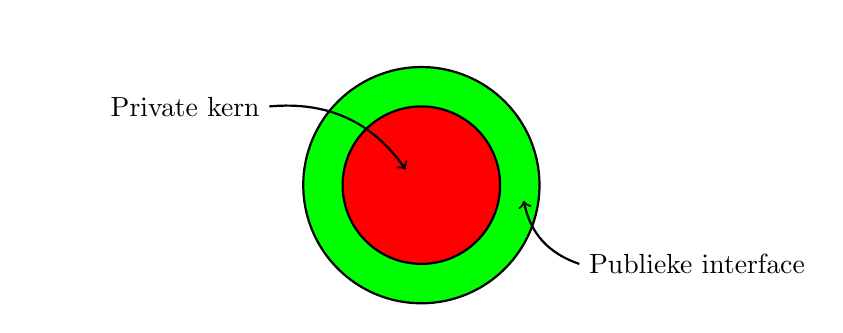
\begin{tikzpicture}
      \path (-5,0) rectangle (5,2);
      \draw[fill=green,thick] (0,0) circle (1.5);
      \draw[fill=red,thick] (0,0) circle (1);
      \node (private) at (-3,1) {Private kern};
      \node (public) at (3.5,-1) {Publieke interface};
      \draw[->,thick,black] (public.west) to [bend left=30] (1.3,-0.2);
      \draw[->,thick,black] (private.east) to [bend left=30] (-0.2,0.2);
    \end{tikzpicture}
  \end{center}
  \begin{itemize}
    \item De complexiteit is verborgen in een \X{\emph{private}}{privatekw} kern
    \item De interface is \X{\emph{publiek}}{publickw} en is en \emph{enige manier} om met het object te interageren
  \end{itemize}
  \begin{tikzpicture}[overlay,
                      remember picture,
                      msg/.style={rectangle,fill=blue!50,opacity=.75,text opacity=1,drop shadow},
                      arr/.style={->,thick}]
    \only<2>{
      \node[msg] (msg) at (8, 0) {{\tt public} en {\tt private} in Java};
      \draw[arr] (msg) to [bend right=30] (publickw);
      \draw[arr] (msg) to [bend right=30] (privatekw);
    }
  \end{tikzpicture}
\end{frame}

\begin{frame}
  \frametitle{Objecten: Velden en Methodes}
  \begin{center}
    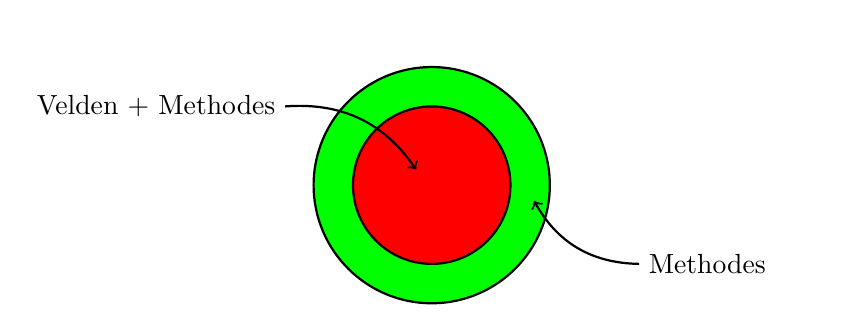
\begin{tikzpicture}
      \path (-5,0) rectangle (5,2);
      \draw[fill=green,thick] (0,0) circle (1.5);
      \draw[fill=red,thick] (0,0) circle (1);
      \node (private) at (-3.5,1) {Velden + Methodes};
      \node (public) at (3.5,-1) {Methodes};
      \draw[->,thick,black] (public.west) to [bend left=30] (1.3,-0.2);
      \draw[->,thick,black] (private.east) to [bend left=30] (-0.2,0.2);
    \end{tikzpicture}
  \end{center}
  \structure{Velden}
  \begin{itemize}
    \item Velden houden de \emph{toestand} van het object bij
    \item Best practice: zijn allemaal private
  \end{itemize}
  \structure{Methodes}
  \begin{itemize}
    \item Methodes bestaan uit algoritmes
    \item Zij manipuleren de toestand van het object
    \item Vormen de publieke interface
  \end{itemize}
\end{frame}

\begin{frame}
  \frametitle{Voorbeeld: Auto}
  \begin{center}
    \begin{tikzpicture}
      \node at (0,0) { \pgfimage[height=2cm,interpolate=true]{carint} };
    \end{tikzpicture}
  \end{center}
  \begin{columns}[t]
    \column{.5\textwidth}
    \structure{Velden}
    \begin{itemize}
      \item<1-> Snelheid
      \item<4-> Versnelling
      \item<5-> Lichten
      \item<6-> Ruitenwissersnelheid
      \item<6-> Knipperlichten
      \item<6-> Merk
      \item<6-> Model
      \item<6-> \dots
    \end{itemize}

    \column{.5\textwidth}
    \structure{Methodes}
    \begin{itemize}
      \item<2-> Versnel
      \item<3-> Rem
      \item<4-> Schakel
      \item<5-> Zet lichten aan/uit
      \item<6-> Zet ruitenwissersstand
      \item<6-> Claxoneer
      \item<6-> Activeer knipperlichten
      \item<6-> \dots
    \end{itemize}
  \end{columns}
\end{frame}

\begin{frame}
  \frametitle{Voorbeeld: Televisie}
  \begin{center}
    \begin{tikzpicture}
      \node at (0,0) { \pgfimage[height=2cm,interpolate=true]{remote} };
    \end{tikzpicture}
  \end{center}
  \begin{columns}[t]
    \column{.5\textwidth}
    \structure{Velden}
    \begin{itemize}
      \item \alt<1>{???}{Kanaal}
      \item<2-> Volume
      \item<2-> Helderheid
      \item<2-> Contrast
      \item<2-> \dots
    \end{itemize}

    \column{.5\textwidth}
    \structure{Methodes}
    \begin{itemize}
      \item     \alt<1>{???}{Verander kanaal}
      \item<2-> Verander volume
      \item<2-> Mute
      \item<2-> Verander contrast
      \item<2-> \dots
    \end{itemize}
  \end{columns}
\end{frame}

\begin{frame}
  \frametitle{Re\"eel Voorbeeld: {\tt MediaPlayer} in Android API}
  \begin{columns}[t]
    \column{.5\textwidth}
    \structure{Velden}
    \begin{itemize}
      \item \X{???}{fields}
    \end{itemize}

    \column{.5\textwidth}
    \structure{Methodes}
    \begin{itemize}
      \item {\tt getCurrentPosition}
      \item {\tt getDuration}
      \item {\tt getVideoHeight}
      \item {\tt getVideoWidth}
      \item {\tt isPlaying}
      \item {\tt seekTo}
      \item {\tt setDataSource}
      \item {\tt pause}
      \item {\tt start}
      \item {\tt stop}
      \item \dots
    \end{itemize}
  \end{columns}
  \vskip4mm
  {\tiny (zie \url{http://developer.android.com/reference/android/media/MediaPlayer.html})}
  \begin{tikzpicture}[overlay,
                      remember picture,
                      msg/.style={rectangle,fill=blue!50,opacity=.75,text opacity=1,drop shadow},
                      arr/.style={->,thick}]
    \node[msg,xshift=2cm,yshift=-1cm] (msg) [below of=fields] {\parbox{5cm}{
        \begin{itemize} 
          \item Velden staan niet in documentatie
          \item Maken deel uit van private kern
        \end{itemize}}};
    \draw[arr] (msg) to [bend right=30] (fields);
  \end{tikzpicture}
\end{frame}

\begin{frame}
  \frametitle{Types}
  \begin{itemize}
    \item Java is \emph{statisch getypeerd}
    \item Velden en methodes annoteren met \emph{types}
    \item JavaScript is \emph{dynamisch getypeerd}: geen types nodig
    \item Type bepaalt welke operaties mogelijk zijn
    \item Terug naar onze voorbeelden\dots
  \end{itemize}
\end{frame}

\begin{frame}
  \frametitle{Types: Velden}
  \begin{center}
    \begin{tikzpicture}
      \node at (0,0) { \pgfimage[height=2cm,interpolate=true]{carint} };
    \end{tikzpicture}
  \end{center}
  \structure{Velden}
  \begin{itemize}
    \item \X{Snelheid}{speed}\only<2->{: \alert<2>{{\tt double}}}
    \item \X{Versnelling}{gear}\only<3->{: \alert<3>{{\tt int}}}
    \item \X{Lichten}{lights}\only<4->{: \alert<4>{{\tt boolean}}}
    \item \X{Ruitenwissersnelheid}{wipers}\only<5->{: \alert<5>{{\tt int}}}
    \item \X{Knipperlichten}{turn}\only<6->{: \alert<6>{{\tt boolean}}}
    \item \X{Merk}{brand}\only<7->{: \alert<7>{{\tt String}}}
    \item \X{Model}{model}\only<8->{: \alert<8>{{\tt String}}}
  \end{itemize}
  \begin{tikzpicture}[overlay,
                      remember picture,
                      msg/.style={rectangle,fill=blue!50,opacity=.75,text opacity=1,drop shadow},
                      arr/.style={->,thick}]
    \only<1>{
      \node[msg,anchor=west] (msg speed) at (5,2.5) {\parbox{6cm}{\raggedright
          Snelheid is een \emph{getal}. Java biedt twee soorten getallen:
          gehele getallen en kommagetallen. We kiezen hier voor kommagetallen.
          In Java heten deze {\tt double}.
      }};
      \draw[arr] (msg speed) to [bend right=30] (speed.east);
    }

    \only<3>{
      \node[msg,anchor=west] (msg gear) at (5,2.5) {\parbox{6cm}{\raggedright
          Het veld ``versnelling'' is duidelijk een geheel getal
          (we kunnen niet naar 2.3de versnelling schakelen).
          In Java heten gehele getallen {\tt int} (kort voor integer).
      }};
      \draw[arr] (msg gear) to [bend right=30] (gear.north);
    }

    \only<4>{
      \node[msg,anchor=west] (msg lights) at (5,2.5) {\parbox{6cm}{\raggedright
          De lichten kunnen aan of uit staan. Wanneer er slechts twee mogelijke
          waarden zijn, worden deze typisch voorgesteld door
          {\tt true} en {\tt false}, en is het type {\tt boolean}.
      }};
      \draw[arr] (msg lights) to [bend right=30] (lights.north);
    }

    \only<5>{
      \node[msg,anchor=west] (msg wipers) at (5,2.5) {\parbox{6cm}{\raggedright
          Voor het veld ruitenwissersnelheid zullen we voor de eenvoud
          kiezen voor {\tt int}.
      }};
      \draw[arr] (msg wipers) to [bend right=30] (wipers.north);
    }

    \only<6>{
      \node[msg,anchor=west] (msg turn) at (5,2.5) {\parbox{6cm}{\raggedright
          We splitsen het veld ``knipperlichten'' op in ``linker-'' en
          ``rechterknipperlicht''. Beide velden hebben dan als type {\tt boolean}.
      }};
      \draw[arr] (msg turn) to [bend right=30] (turn.north);
    }

    \only<7>{
      \node[msg,anchor=west] (msg brand) at (5,2.5) {\parbox{6cm}{\raggedright
          Het merk kan niet voorgesteld worden door een getal,
          en er zijn zeker meer dan twee mogelijke waarden.
          In dit geval kunnen we beroep doen op het type {\tt String}:
          dit is een rij tekens.
      }};
      \draw[arr] (msg brand.west) to [bend right=30] (brand.north);
    }

    \only<8>{
      \node[msg,anchor=west] (msg model) at (5,2.5) {\parbox{6cm}{\raggedright
          Model kunnen we best ook het type {\tt String} toekennen.
      }};
      \draw[arr] (msg model.west) to [bend right=30] (model.north);
    }
  \end{tikzpicture}
\end{frame}

\begin{frame}
  \frametitle{Voorbeeld: Televisie}
  \begin{center}
    \begin{tikzpicture}
      \node at (0,0) { \pgfimage[height=2cm,interpolate=true]{remote} };
    \end{tikzpicture}
  \end{center}
  \begin{columns}[t]
    \column{.5\textwidth}
    \structure{Velden}
    \begin{itemize}
      \item Kanaal: \alt<1>{???}{\alert<2>{\tt int}}
      \item Volume: \alt<1>{???}{\alert<2>{\tt int}}
      \item Helderheid: \alt<1>{???}{\alert<2>{\tt int}}
      \item Contrast: \alt<1>{???}{\alert<2>{\tt int}}
    \end{itemize}
    \column{.5\textwidth} \only<2>{\phantom{bla}}
  \end{columns}
\end{frame}

\begin{frame}
  \frametitle{Types}
  \structure{Beschikbare (primitieve) types}
  \begin{itemize}
    \item Gehele getallen: {\tt byte}, {\tt short}, \alert{\tt int}, {\tt long}
    \item Kommagetallen: {\tt float}, \alert{\tt double}
    \item Booleaanse waarden: \alert{\tt boolean}
    \item Enkel teken: \alert{\tt char}
    \item Reeks tekens: \alert{\tt String}
  \end{itemize}
  \vskip4mm
  In rood aangeduide types zijn meest gebruikte.
\end{frame}

\begin{frame}
  \frametitle{Types van Methodes}
  \begin{itemize}
    \item Methodes zijn ingewikkelder dan velden
    \item Methodes kunnen \emph{parameters} meekrijgen
    \item Elke parameter heeft een bepaald type
    \item Een methode kan een resultaat opleveren
    \item Een methode heeft een returntype
    \item Speciaal type voor methodes die niks zinvol kunnen teruggeven: {\tt void}
  \end{itemize}
\end{frame}

\begin{frame}
  \frametitle{Voorbeeld: Auto}
  \begin{center}
    \begin{tikzpicture}
      \node at (0,0) { \pgfimage[height=2cm,interpolate=true]{carint} };
    \end{tikzpicture}
  \end{center}
  \structure{Methodes}
  \begin{itemize}
    \item \alt<1>{Schakel}{\alert<2>{{\tt void schakel(int versnelling)}}}
    \item \alt<1-3>{Zet lichten aan/uit}{\alert<4>{\tt void zetLichten(boolean aan)}}
    \item \alt<1-5>{Claxoneer}{\alert<6>{\tt void claxoneer()}}
    \item \alt<1-7>{Welk merk?}{\alert<8>{\tt String geefMerk()}}
  \end{itemize}
  \begin{tikzpicture}[overlay,
                      remember picture,
                      msg/.style={rectangle,fill=blue!50,opacity=.75,text opacity=1,drop shadow},
                      arr/.style={->,thick}]
    \only<1>{
      \node[msg,anchor=west] at (5,1.5) {\parbox{6cm}{\raggedright
          Als we schakelen, is dit altijd naar een bepaalde versnelling.
          We kunnen dit als parameter meegeven: het type is {\tt int}
          en de naam is {\tt versnelling}.
      }};
    }

    \only<3>{
      \node[msg,anchor=west] at (5,1.5) {\parbox{6cm}{\raggedright
          Het aan- en uitzetten van de lichten kan met een enkele methode;
          het hoeft enkel te weten of we de lichten wens aan- of uit te zetten.
          Dit gaat via een parameter van het type {\tt boolean}.
          Lichten aanzetten gaat dan met {\tt zetLichten(true)}.
      }};
    }

    \only<5>{
      \node[msg,anchor=west] at (5,1.5) {\parbox{6cm}{\raggedright
          Claxoneren heeft geen parameters nodig.
      }};
    }

    \only<7>{
      \node[msg,anchor=west] at (5,1.5) {\parbox{6cm}{\raggedright
          Het merk opvragen moet via een methode (velden zijn private).
          De methode moet een resultaat opleveren, nl.\ het merk.
          Dit betekent dat de methode returntype {\tt String} moet hebben.
      }};
    }

    \only<8>{\phantom{foo}}
  \end{tikzpicture}
\end{frame}

\begin{frame}
  \frametitle{{\tt MediaPlayer} in Android API}
  \structure{Methodes}
  \begin{overprint}
    \onslide<1>
    \begin{itemize}
      \item {\tt getCurrentPosition}
      \item {\tt getDuration}
      \item {\tt getVideoHeight}
      \item {\tt getVideoWidth}
      \item {\tt isPlaying}
      \item {\tt seekTo}
      \item {\tt setDataSource}
      \item {\tt pause}
      \item {\tt start}
      \item {\tt stop}
    \end{itemize}

    \onslide<2>
    \begin{itemize}
      \item {\tt int getCurrentPosition()}
      \item {\tt int getDuration()}
      \item {\tt int getVideoHeight()}
      \item {\tt int getVideoWidth()}
      \item {\tt boolean isPlaying()}
      \item {\tt void seekTo(int msec)}
      \item {\tt void setDataSource(String path)}
      \item {\tt void pause()}
      \item {\tt void start()}
      \item {\tt void stop()}
    \end{itemize}
  \end{overprint}
  \vskip2mm
  Ter herinnering: types zijn {\tt int}, {\tt double}, {\tt boolean}, {\tt char}, {\tt String}
\end{frame}

\begin{frame}
  \frametitle{Klassen}
  \begin{itemize}
    \item Objecten bevatten velden en methodes
    \item In de praktijk willen we vaak meerdere dezelfde objecten aanmaken
    \item Elk object heeft zijn eigen toestand en dezelfde interface
  \end{itemize}
  \begin{center}
    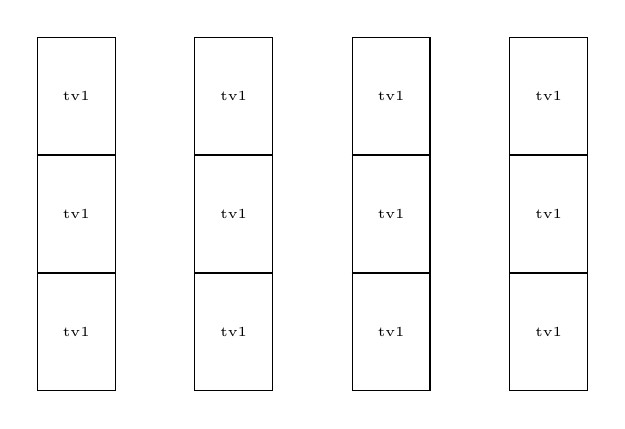
\begin{tikzpicture}
      \foreach \posy in {0,1.5,3} {
        \foreach \posx in {0,2,4,6} {
          \node at (\posx, \posy) { \pgfimage[height=1.5cm,interpolate=true]{tv1} };
        };
      };
    \end{tikzpicture}
  \end{center}
\end{frame}

\begin{frame}
  \frametitle{Klassen}
  \begin{itemize}
    \item ``Gelijke'' objecten behoren tot eenzelfde \emph{klasse}
    \item In Java moet men eerst de klasse defini\"eren
    \item Deze definieert velden en methodes
    \item Men kan dan in een tweede stap deze klasse \emph{instanti\"eren}, dit levert een object op
    \item De klasse is de blauwdruk voor objecten
  \end{itemize}
  \begin{center}
    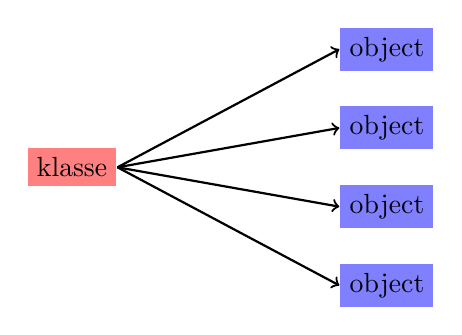
\begin{tikzpicture}[class/.style={rectangle,fill=red!50,thick},
                        object/.style={rectangle,fill=blue!50,thick},
                        arr/.style={->,thick}]
      \node[class] (class) at (0,1.5) { klasse };
      \foreach \idx in {0,1,2,3} {
        \node[object] (object\idx) at (4,\idx) { object };
        \draw[arr] (class.east) -- (object\idx.west);
      };      
    \end{tikzpicture}
  \end{center}
\end{frame}

\begin{frame}
  \frametitle{Actuele Code voor TV}
  \codeblock[basicstyle={\small\tt}]{tv.java}{TV}
\end{frame}

\begin{frame}
  \frametitle{Actuele Code voor MediaPlayer}
  \codeblock[basicstyle={\small\tt}]{mediaplayer.java}{MediaPlayer}
\end{frame}

\begin{frame}
  \frametitle{Oefening: Tally Counter}
  \begin{columns}
    \column{.4\textwidth}
    \begin{center}
      \begin{tikzpicture}
        \node { \pgfimage[height=4cm,interpolate=true]{counter} };
      \end{tikzpicture}
    \end{center}

    \column{.6\textwidth}
    \structure{Tally Counter}
    \begin{itemize}
      \item Teller
      \item Druk op de knop om met 1 te verhogen
    \end{itemize}
    \vskip5mm
    \structure{Opgave}
    \begin{itemize}
      \item Wat zijn de velden en hun types?
      \item Wat zijn de methodes?
    \end{itemize}
  \end{columns}
\end{frame}

\begin{frame}
  \frametitle{Oefening: Tally Counter}
  \codeblock[basicstyle={\small\tt}]{counter.java}{Counter}  
\end{frame}

\begin{frame}
  \frametitle{Oefening: Tally Counter}
  \codeblock[basicstyle={\small\tt}]{counter2.java}{Counter met method bodies}
  Voeg een {\tt reset} methode toe (zet teller terug op 0).
\end{frame}

\begin{frame}
  \frametitle{Oefening: Tally Counter}
  \codeblock[basicstyle={\small\tt}]{counter3.java}{Counter met {\tt reset}}
  Voeg een {\tt setCount} methode toe die de teller op een willekeurig getal kan instellen.
\end{frame}

\begin{frame}
  \frametitle{Oefening: Tally Counter}
  \codeblock[basicstyle={\small\tt}]{counter4.java}{Counter met {\tt setCount}}  
  We kunnen deze code verbeteren.
\end{frame}

\begin{frame}
  \frametitle{Oefening: Tally Counter}
  \codeblock[basicstyle={\small\tt}]{counter5.java}{Verbeterde Counter}
\end{frame}



%%% Local Variables: 
%%% mode: latex
%%% TeX-master: "intro"
%%% End: 
